%\documentclass[11pt,a4paper]{report}


% The Beamer class comes with a number of default slide themes
% which change the colors and layouts of slides. Below this is a list
% of all the themes, uncomment each in turn to see what they look like.

%\usetheme{default}
%\usetheme{AnnArbor}
%\usetheme{Antibes}
%\usetheme{Bergen}
%\usetheme{Berkeley}
%\usetheme{Berlin}
%\usetheme{Boadilla}
%\usetheme{CambridgeUS}
%\usetheme{Copenhagen}
%\usetheme{Darmstadt}
%\usetheme{Dresden}
%\usetheme{Frankfurt}
%\usetheme{Goettingen}
%\usetheme{Hannover}
%\usetheme{Ilmenau}
%\usetheme{JuanLesPins}
%\usetheme{Luebeck}
%\usetheme{Madrid}
%\usetheme{Malmoe}
%\usetheme{Marburg}
%\usetheme{Montpellier}
%\usetheme{PaloAlto}
%\usetheme{Pittsburgh}
%\usetheme{Rochester}
%\usetheme{Singapore}
%\usetheme{Szeged}
%\usetheme{Warsaw}

\documentclass[10pt]{beamer}
\usepackage{float}
\usepackage[nodisplayskipstretch]{setspace}
\usepackage{pdfpages}
\usepackage{tikz}    
\usetheme{metropolis}
\usepackage{appendixnumberbeamer}
\usepackage[normalem]{ulem}
\usepackage{eurosym}
\usepackage{booktabs}
\usepackage[scale=2]{ccicons}
\usepackage[utf8]{inputenc}
\usepackage{soul}
\usepackage{mathabx}
\usepackage{graphicx}
\usepackage{pgfplots}
\usepgfplotslibrary{dateplot}
 \usepackage{relsize}
\usepackage{xspace}
\usepackage{caption}

\usepackage{graphicx}
\usepackage{graphicx}

\usepackage{hyperref}
\hypersetup{
    colorlinks=true,
    linkcolor=blue,
    filecolor=magenta,      
    urlcolor=blue,
}
 
\urlstyle{same}
\newcommand{\themename}{\textbf{\textsc{metropolis}}\xspace}


% As well as themes, the Beamer class has a number of color themes
% for any slide theme. Uncomment each of these in turn to see how it
% changes the colors of your current slide theme.

%\usecolortheme{albatross}
%\usecolortheme{beaver}
%\usecolortheme{beetle}
%\usecolortheme{crane}
%\usecolortheme{dolphin}
%\usecolortheme{dove}
%\usecolortheme{fly}
%\usecolortheme{lily}
%\usecolortheme{orchid}
%\usecolortheme{rose}
%\usecolortheme{seagull}
%\usecolortheme{seahorse}
%\usecolortheme{whale}
%\usecolortheme{wolverine}

%\setbeamertemplate{footline} % To remove the footer line in all slides uncomment this line
%\setbeamertemplate{footline}[page number] % To replace the footer line in all slides with a simple slide count uncomment this line

%\setbeamertemplate{navigation symbols}{} % To remove the navigation symbols from the bottom of all slides uncomment this line


\usepackage[utf8]{inputenc}
\usepackage{graphicx}

\usepackage{amsmath,amsthm,amssymb,latexsym,amsfonts}
\usepackage{tikz}
\newcommand*\circled[1]{\tikz[baseline=(char.base)]{
   \node[shape=circle,color=red,draw,inner sep=1pt] (char) {#1};}}


\setlength{\parindent}{15pt}
\usepackage{subfig}
\usepackage{hyperref}
\usepackage{graphicx} % Allows including images
\usepackage{booktabs} % Allows the use of \toprule, \midrule and \bottomrule in tables

\usepackage{bm}

\newtheorem{caution}[theorem]{¡Cuidado!}

\def\Q{\mathbb{Q}}
\def\R{\mathbb{R}}
\def\C{\mathbb{C}}
\def\N{\mathbb{N}}
\def\Z{\mathbb{Z}}
\def\S{\mathcal{S}}
\def\H{\mathcal{H}}
%\def\sde{\underset{\theta}{\times}}
\def\sde#1{\underset{#1}{\times}}

\def\G{Sea $G$ un grupo}
\def\GG{Sean\ $G, G'$\ grupos}
\def\GS{Sea\ $G$ un grupo y $S\in\S(G)$}
\def\ac{Sea $\cdot: G\times X \rightarrow X$ una acción}

\def\dcup{\sqcup}

\def\gen#1{<#1>}
\def\genn#1{<\bar{#1}>}
\def\key#1{\{#1\}}

%tetration
\def\inv#1#2{(#2,#1)}

\def\ii{\textbf{i}}
\def\jj{\textbf{j}}
\def\kk{\textbf{k}}

\def\div{por el algoritmo de división, existen $q,r$ tal que\xspace}
\def\Div{Por el algoritmo de división, existen $q,r$ tal que\xspace}
\def\m{^{-1}}

%Cambiar por un triangulito
\def\n{\Delta}

\def\p{Sea $p$ un número primo}

\def\I{[a,b]} 


\usepackage[utf8]{inputenc}
\usepackage{graphicx}
\graphicspath{ {images/} }

\usepackage[export]{adjustbox}
\usepackage{hyperref}
\usepackage{graphicx} % Allows including images
\usepackage{booktabs} % Allows the use of \toprule, \midrule and \bottomrule in tables

\usepackage{etoolbox}

\addtobeamertemplate{proof begin}{%
	\setbeamercolor{block title}{fg=black,bg=red!50!white}
	\setbeamercolor{block body}{fg=red, bg=red!30!white}
}{}


\BeforeBeginEnvironment{definition}{
	\setbeamercolor{block title}{fg=black,bg=green!20!gray}
	%\setbeamercolor{block body}{fg=black, bg=green!40!gray}
}

\AfterEndEnvironment{definition}{
	\setbeamercolor{block title}{fg=black,bg=green!20!gray}
	%\setbeamercolor{block body}{fg=black, bg=green!40!gray}
}

\BeforeBeginEnvironment{theorem}{
	\setbeamercolor{block title}{fg=black,bg=gray!40!white}
	%\setbeamercolor{block body}{fg=black, bg=green!40!gray}
}

\AfterEndEnvironment{theorem}{
	\setbeamercolor{block title}{fg=black,bg=gray!40!white}
	%\setbeamercolor{block body}{fg=black, bg=green!40!gray}
}



\title{Cuaterniones}


\begin{document}

\maketitle


\begin{frame}{¿Qué es una rotación?}

% Antes de empezar estaría bueno ponernos de acuerdo en la respuesta a esta pregunta: ¿qué es una rotación?

¿...?

% Hay definiciones de rotaciones bien matemáticas, formales, generales, que no nos interesan. Sin embargo, distingamos un par de propiedades de las rotaciones

\pause

\begin{itemize}
	\item Después de una rotación, los cuerpos rígidos mantienen su forma. % Rotan todos juntos	
	%\item Preservan la orientación de los objetos.
	\item Siempre hay un punto que queda quieto en el sistema de referencia, al que llamamos origen, o centro.
\end{itemize}

% El objetivo de la charla va a ser entender las rotaciones de una manera más "abstracta", usando  números complejos, matrices y finalmente cuaterniones. Pero también al revés: dado alguno de estos objetos matemáticos, vamos a querer imaginarnos la rotación que representan.


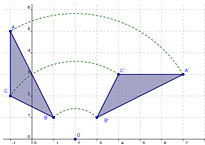
\includegraphics[scale=0.8]{rigid.png}
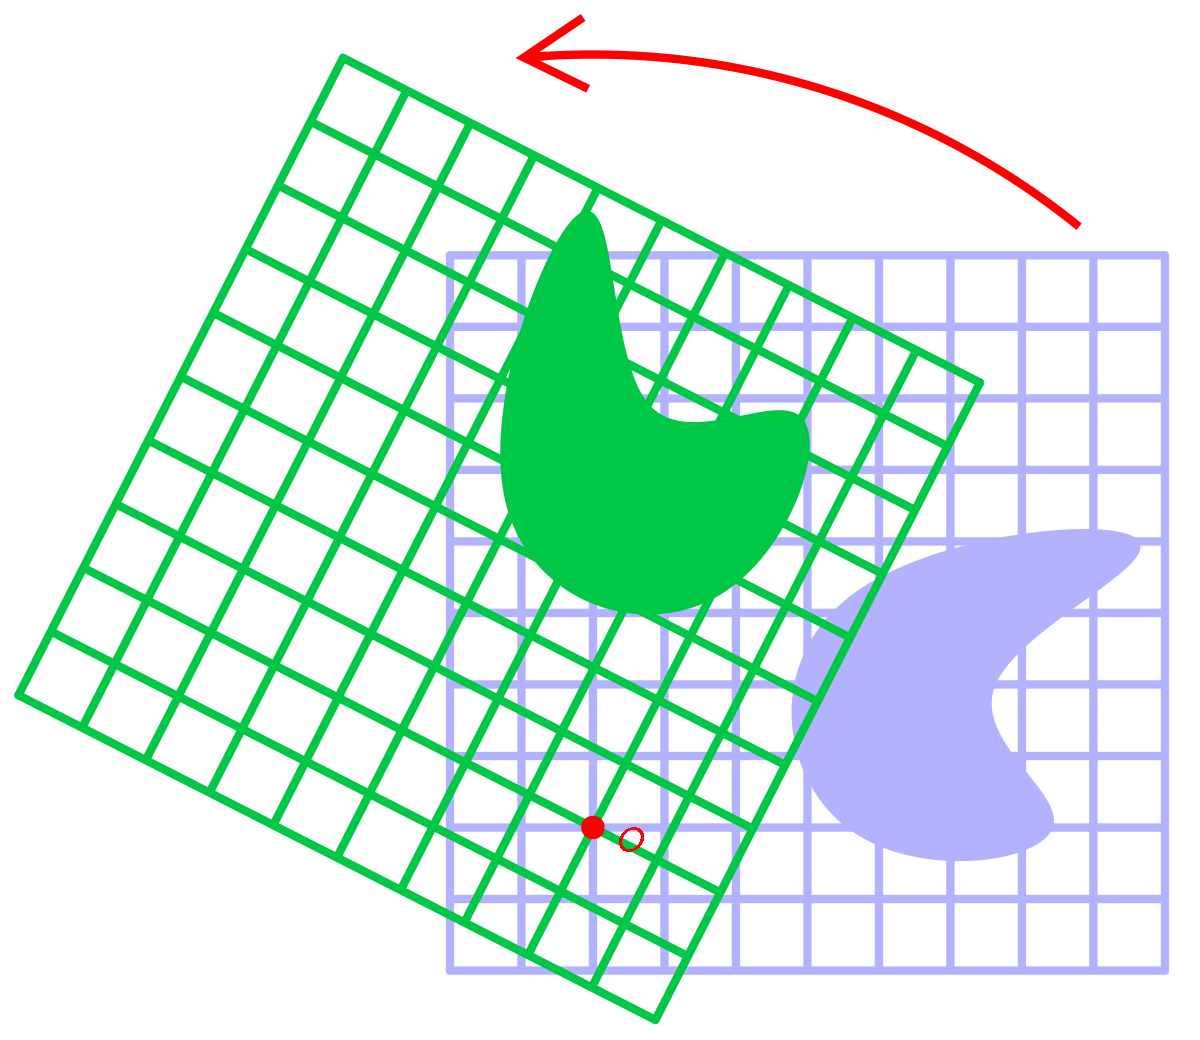
\includegraphics[scale=0.11]{fixed.png}

\end{frame}

\begin{frame}{Rotaciones en $2D$: con números complejos}

% Empecemos por las rotaciones en $\R^2$, que son más fáciles. ¿Cómo son? ¿Cómo se describen? ¿Cómo hago para [PIZARRÓN] armar una rotación (con centro en el origen) que mueva un punto $P$ a un punto $Q$ (de la misma longitud)?

% Acá los números complejos nos van a resultar muy útiles. Así que veamos qué eran.

Empecemos por las rotaciones en $2D$, usando números complejos. \bigskip

\pause

%TODO agregar imagen de conjuntos aritméticos y dejar eso en vez de esto:
\small{Nats $\rightarrow$ Enteros (tienen negativos)}

Reales $\rightarrow$ Complejos ($\rightarrow$ ¡Cuaterniones!) \pause \bigskip

¿Cuánto vale $\sqrt{-1}$?\pause\ Bueno, llamémoslo $\ii$ \pause


¿Y qué hacemos con eso? ¿Cómo hacemos cuentas?

% Los números complejos no son nada más que un "upgrade" que led hacemos a los números que ya teníamos. En la primaria empezamos con los naturales, después nos preguntamos qué pasaba si le restábamos un número más grande a un número más chico y aparecieron los enteros, que son los que también pueden ser negativos, y para responder preguntas similares nos inventamos a los números racionales y a los reales, que son los qué conocemos más o menos bien.

% Los números complejos aparecen al responder la pregunta: "cuánto vale \sqrt{-1}"?


%PIZARRÓN: $i^2=-1$.

% Es una abstracción más, así como los números negativos son una abstracción a la que ya estamos super acostumbrados. Y...es una abstracción súper útil.

% Ahora que nos inventamos un nuevo número \textbf{i}, podemos sumarlo y multiplicarlo por otros números, obteniendo:

% PIZARRÓN: 1+i, 2+i, 3\cdot i, 2 + 3\cdot i

% Y podemos preguntarnos qué representan esos nuevos números

\end{frame}



\begin{frame}{Números complejos en el plano}

	%Y resulta que también es útil representar a los números complejos en un plano, como si tuvieran dos coordenadas. Veamos el siguiente ejemplo.
	\includegraphics[scale=0.8]{1plusi.png}
	
	% Como $i^2=-1$
	% Fíjense que cuando hacemos esto, les podemos inventar dos características nuevas a los números complejos:
	\pause
	
	\begin{itemize}
	
		% Pitágoras
		\item Longitud ('módulo'): $|1+\ii| = \sqrt{1^2 + |\ii|^2} = \sqrt{1+1} = \sqrt{2}$

		% Trigonometría, SOHCAHTOA		
		\item Ángulo: $\alpha = cos\m(\frac{CA}{HIP}) = cos\m(\frac{1}{\sqrt{2}}) = 45^\degree = \frac{\pi}{4}$
	\end{itemize}
\end{frame}

\iffalse
\begin{frame}{Conjugación}

$$x = a+b\cdot \textbf{i} \Rightarrow x^* (=\bar{x}) = a\circled{-}b\cdot \textbf{\ii}$$

% A los números complejos se los puede conjugar

% Es cambiar el signo del numerito que acompaña a \textbf{i}
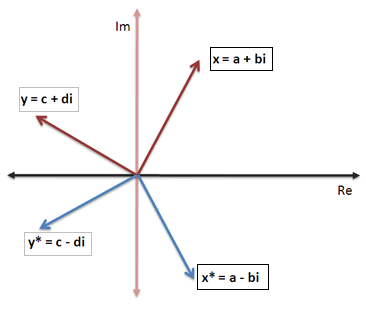
\includegraphics[scale=0.8]{conjugado.png}

%TODO ¿por qué es buena la conjugación? Porque nos re sirve para obtener inversos

\end{frame}
\fi


\begin{frame}{Forma trigonométrica}

¡Tener un número complejo es lo mismo que tener su ángulo y su módulo!
	% Copio el dibujo en el pizarrón y hago trigonometría para probar la forma trigonométrica
	
	% SOH. sen(\alpha) = \frac{CO}{HIP} \Rightarrow CO = sen(\alpha) HIP = sen(\alpha) |z|
	% CAH. cos(\alpha) = \frac{CA}{HIP} \Rightarrow CA = cos(\alpha) HIP = cos(\alpha) |z|
	
	% Entonces si tengo z = a+bi, CA = a, CO = b, y sacando factor común obtenemos...
	
	De hecho si el número es $a + b\cdot i$ entonces:
	
	$$cos(\text{ángulo}) \cdot \text{longitud} = a$$
	$$sen(\text{ángulo}) \cdot \text{longitud} = b$$
	
\iffalse
\[
	z = a + b\cdot i = \text{longitud} \cdot [\underbrace{cos(\text{ángulo})}_{a/HIP} + \ii\cdot \underbrace{sen(\text{ángulo})}_{b/HIP}]
\]

Escrito con letras:

\[
	z = a + b\cdot i = |z| \cdot [\underbrace{cos(\alpha)}_{a/HIP} + \ii\cdot \underbrace{sen(\alpha)}_{b/HIP}]
\]

\fi
\end{frame}


\begin{frame}{¿Cómo operar?}
	% Algo que pasa y que se puede demostrar con más trigonometría pero que no vamos a hacer es que cuando multiplicamos dos números complejos, lo que obtenemos es un nuevo número complejo donde los módulos se multiplican y los ángulos se suman
	
	Si $z,w$ son complejos, entonces $z \cdot w$ 'es' sumar los ángulos y multiplicar las longitudes (los 'modulos'). \pause
	
	
	
	¡Hagamos un ejemplo! ¿Cuánto da $(1+\ii)\cdot \i$?
	
%	Si $z = |z|\cdot [cos(\alpha) + \ii\cdot sen (\alpha)]$,\\
%	   $w = |w|\cdot [cos(\beta) + \ii\cdot sen (\beta)]$ \\
%	   entonces $z\cdot w = |z|\cdot |w|\cdot [cos(\alpha+\beta) + \ii \cdot sen(\alpha+\beta)]$
	   
	   % O sea, el módulo del nuevo número complejo es $|z||w|$, y el ángulo es $\alpha+\beta$
	   
	   % Un buen ejemplo es i^2=-1 (el módulo es 1 y el ángulo pasa de pi/2 a pi)
\end{frame}


\begin{frame}

\Huge{Muy lindo, ¿pero y con las rotaciones qué onda?}

Pensemos un poco cómo se relacionan.

% Fíjense qué bueno: si agarramos a un número complejo y lo multiplicamos por otro de módulo $1$, ¡lo estamos rotando! porque el módulo del primer complejo no cambia pero su ángulo sí.

%Hacer ejemplo en el pizarrón: 1\cdot i, (1+i) \cdot i$

\end{frame}

\begin{frame}{Ejemplo}

¿Cómo llevo el punto $(1,1)$ al punto  $(-\sqrt{2},0)$?

% PIZARRÓN dibujar
% Fíjense que necesito que los dos tengan el mismo módulo (la misma longitud), sino el problema es imposible.

% Se puede obtener el ángulo de 1+i con trigonometría pero es aburrido y además existen funciones que ya te lo hacen.

% Necesito ángulo 3/4 pi, entonces lo escribo en forma trigonométrica y listo.
\end{frame}

%TODO tal vez otra imagen sería mejor
\begin{frame}

% Los complejos de módulo 1 representan rotaciones, y fíjense que si tenés modulo 1 estás en la circunferencia de radio 1. En ese sentido el número complejo indica qué rotación es.
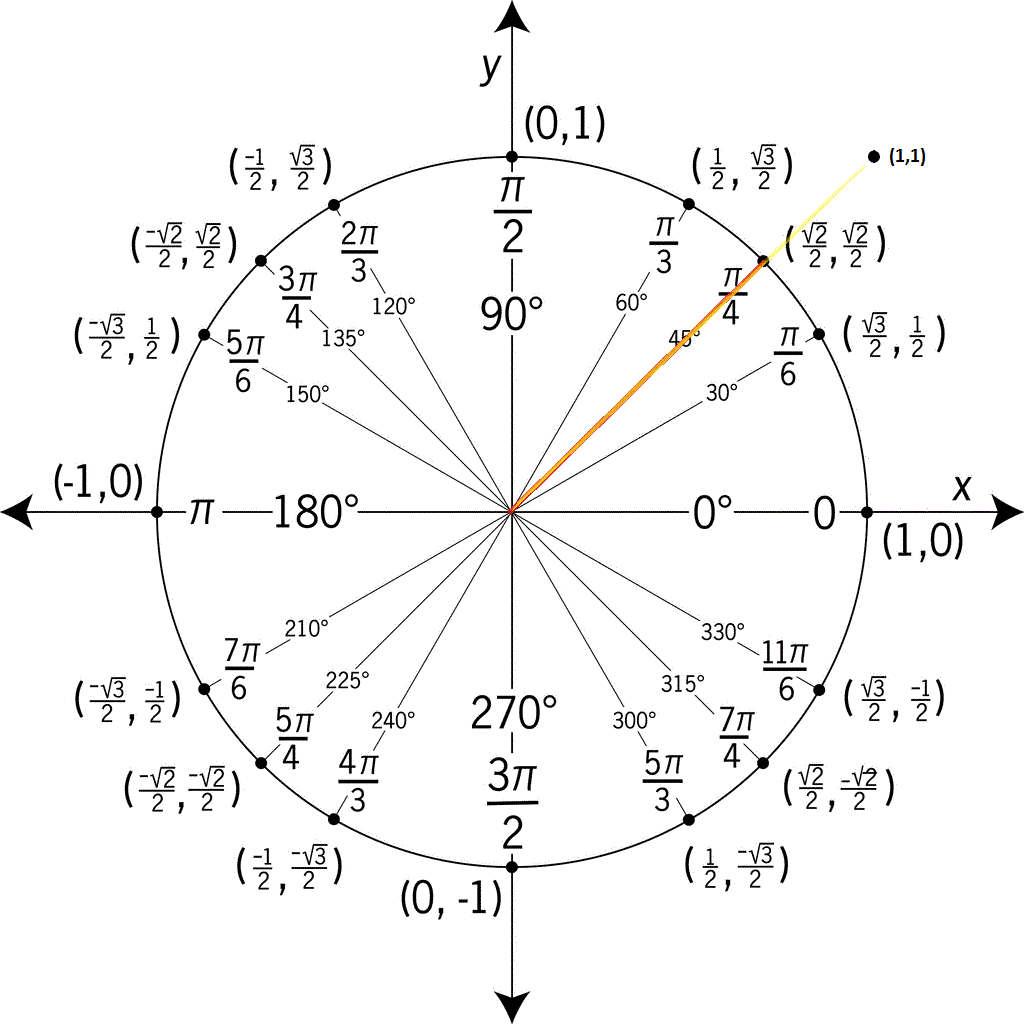
\includegraphics[scale=0.35]{unit_circle.png}

\end{frame}

\begin{frame}{¿Cómo invierto una rotación?}

%TODO Expandir
¿Será difícil? \pause

Si tengo $a+b\cdot \textbf{i}$ con ángulo $\alpha$ y quiero otro número complejo con ángulo $-\alpha = 2\pi - \alpha$, lo conjugo, es decir, uso $a-b\cdot\textbf{i}$

\begin{figure}
\centering
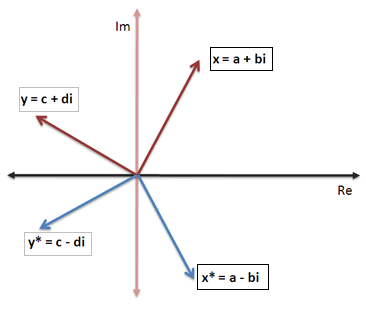
\includegraphics[scale=0.7]{conjugado.png}
\end{figure}

% Y fíjense qué copado. Cuánto da z \bar{z}? Es posta el inverso! (Si el módulo es 1)

\end{frame}



% Para el final de números complejos
\begin{frame}{Volvamos a \textbf{i}}

¿Cuál es la solución de $x^2=-1$? \pause

% Fíjense que esta ecuación es lo mismo que esta.

$1\cdot x^2 = -1$

% Y ahora la pregunta es: ¿qué rotación, aplicada 2 veces, lleva el 1 a -1?
% Hay que girar 2 \pi, pero haciendo dos veces la misma rotación. O sea, la rotación tiene que ser de \pi, un ángulo recto. Y qué número complejo representa un número recto? i! 

\pause

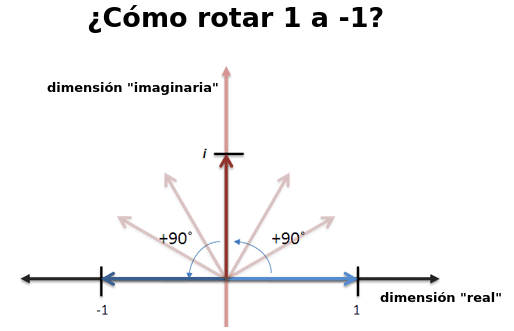
\includegraphics[scale=0.78]{rotate1m1.png}


\end{frame}


\begin{frame}{Volvamos a \textbf{i} (cont)}
	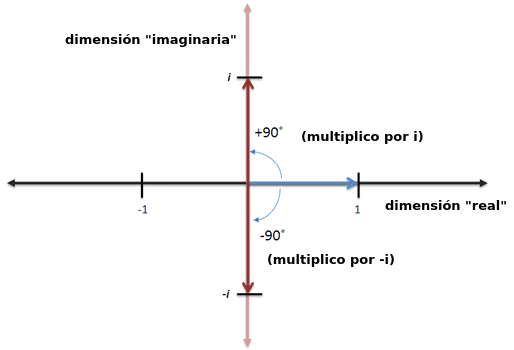
\includegraphics[scale=0.78]{rotate1m1_2.png}
	
	% Y el álgebra nos lo confirma: (-i)\cdot (-i) = (-1) \cdot i \cdot (-1) \cdot i = i \cdot i = 1$. Estamos usando que el producto es conmutativo.
\end{frame}



\iffalse

%TODO hablo de matrices? Sirve para algo?
\begin{frame}{Matrices}

% Bueno, quiero pasar ahora a otra herramienta para entender rotaciones (y más adelante, en particular, a los cuaterniones)

% Hablemos un poco de matrices.



\[
\begin{bmatrix}
    1  &  -1      \\
    0  &  2      
\end{bmatrix}
\visible<2->{\cdot
\begin{bmatrix}
    1  &  0      \\
    0  &  2      
\end{bmatrix} }
\visible<3->{=
\begin{bmatrix}
    1  &  -2      \\
    0  &  4      
\end{bmatrix} }
\]


\end{frame}

\begin{frame}{Matrices}
\[
\begin{bmatrix}
    1  &  -1      \\
    0  &  2      
\end{bmatrix}
\cdot
\begin{bmatrix}
    1  &  0      \\
    0  &  2      
\end{bmatrix}
 =
\begin{bmatrix}
    1  &  -2      \\
    0  &  4      
\end{bmatrix}
\] 

\[
\begin{bmatrix}
    0  &  -1      \\
    1  &  0      
\end{bmatrix}
\cdot
\begin{bmatrix}
      1      \\
      0      
\end{bmatrix}
=
\begin{bmatrix}
    0        \\
    1        
\end{bmatrix}
\]

\end{frame}


\begin{frame}{¿Y para qué sirven?}
Algunas propiedades:
	\begin{itemize}
		\item Representan funciones (transformaciones del espacio).
		\item Los números complejos se pueden ver como matrices
		\item Algunas matrices representan rotaciones
	\end{itemize}
\end{frame}

\begin{frame}{Las matrices como funciones (transformaciones lineales)}

$ A \leftarrow$ matriz

$ x \leftarrow$ punto ('vector') genérico de $\R^2$ (el plano) \bigskip

Puedo definir la siguiente función:

\Huge $$f(x) = A\cdot x$$

% Gracias a que cuando multiplico una matriz por un vector me da otro vector, dada una matriz me puedo definir una función.




\end{frame}


\begin{frame}{Números complejos como matrices}

Si $z=a+bi$, ¡se puede expresar como matriz! \pause

\[
\begin{bmatrix}
    a  &  -b      \\
    b  &  a      
\end{bmatrix}
\]

\begin{itemize}
	\item El producto de complejos se corresponde con el producto de matrices
	\item Todo anda bien
\end{itemize}
	
% Esa matriz guarda la información, con dos valores repetidos, del número complejo. O sea, el número está en la primera columna.

% Y el producto de dos complejos anda bien, veamos un ejemplo

% Que el ejemplo sea (1+i) (i)


	
\end{frame}


\begin{frame}{Algunas matrices son rotaciones}

Esto es una consecuencia de las dos slides anteriores.

Si $z =  \underbrace{cos(\alpha)}_{a} + i \underbrace{\ sen(\alpha)}_{b}$ (o sea, tiene módulo $1$), la matriz que le podemos asociar es:

\[
\begin{bmatrix}
    cos(\alpha)  &  -sen(\alpha)      \\
    sen(\alpha)  &  cos(\alpha)      
\end{bmatrix}
\] \pause

Este tipo de matrices representan las rotaciones en $2D$.

\begin{itemize}
	\item Forman un \textbf{grupo} conmutativo llamado $SO(2)$.
	%\item La inversa de una matriz allí es su transpuesta % Coincide con el inverso del complejo
	\item En particular, todo elemento tiene inverso. %Conviene pensar en rotaciones!
	%\item Tienen determinante $1$. % Coincide con el cuadrado del módulo del número complejo
	
\end{itemize}

% Todas estas propiedades se pueden ver tanto viéndolas como números complejos, como con matrices, o simplemente pensando en rotaciones de $\R^2$

% La idea es que elijan la manera de pensar qué más les guste pero si tienen una manera de pasar de un mundo a otro eso les puede servir para atacar un problema de varias formas distintas

% Si uno piensa un problema con el enfoque que más le conviene, pero el resultado lo tiene que dar en el otro universo, hace la traducción y listo

% Si quieren, por ejemplo, podemos tratar de entender cómo es el inverso de un número complejo de módulo 1, pensando con rotaciones.
\end{frame}

\fi


\begin{frame}{¿Qué es una rotación (en $3D$)?}

	\Huge ¿Qué es una rotación en $3D$?


% Antes de cerrar la charla quiero empezar a hablar un poco de $\R^3$ y que se note la relevancia de todo lo que discutimos en $\R^2$

	
\end{frame}

\begin{frame}{¿Qué es una rotación en $3D$? Formalismo matemático}
	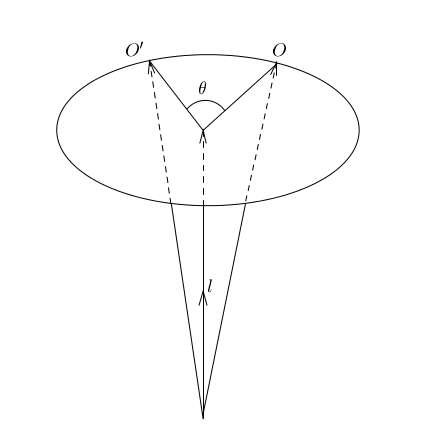
\includegraphics[scale=0.6]{images/rotation.png}
	
	%Una rotación de $\R^3$ está compuesta por un eje $\ell$ (que define un plano ortogonal) y un ángulo $\theta$...y ya sé lo que están pensando. Ese dibujo no se entiende.
	
\end{frame}


\begin{frame}{¿Qué es una rotación en $3D$? Un pisa papas}

%TODO El mango del pisa papas y la rejilla están a 90 grados. Y un pisapapas representa, bien en el fondo, una rotación en $\R^3$. El mango es el eje de rotación y un punto de la rejilla rota alrededor del mango con un ángulo fijo, como si fuera una rotación en $\R^2$ donde el origen está donde el mango y la rejilla se tocan.

%PIZARRÓN: hagamos el dibujito en el pizarrón
% Ojo que el pisa papas debe pasar por el origen! Sino no funciona la cosa

% ¿Cómo gira un punto que no está en la rejilla? Bueno, según una rejilla imaginaria

% Además el pisa papas puede estar inclinado de distintas maneras
	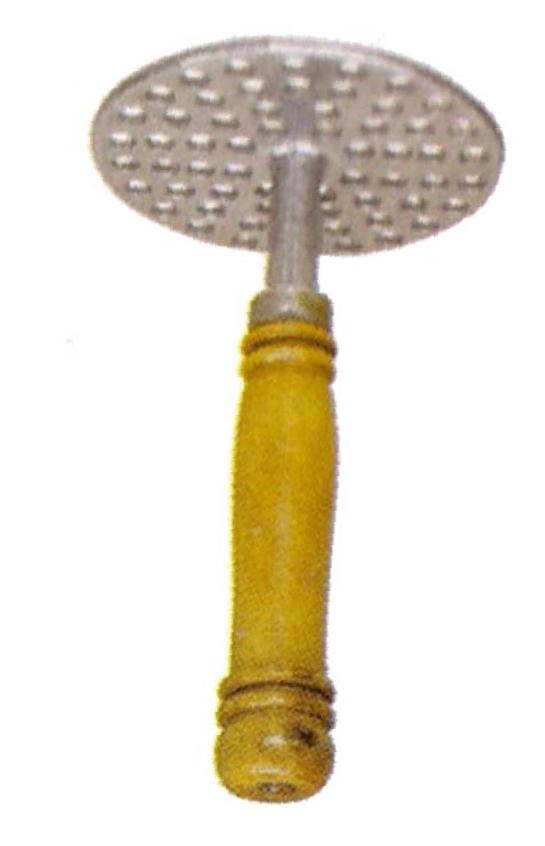
\includegraphics[scale=0.2]{pisapapas_dadovuelta.png} \pause
	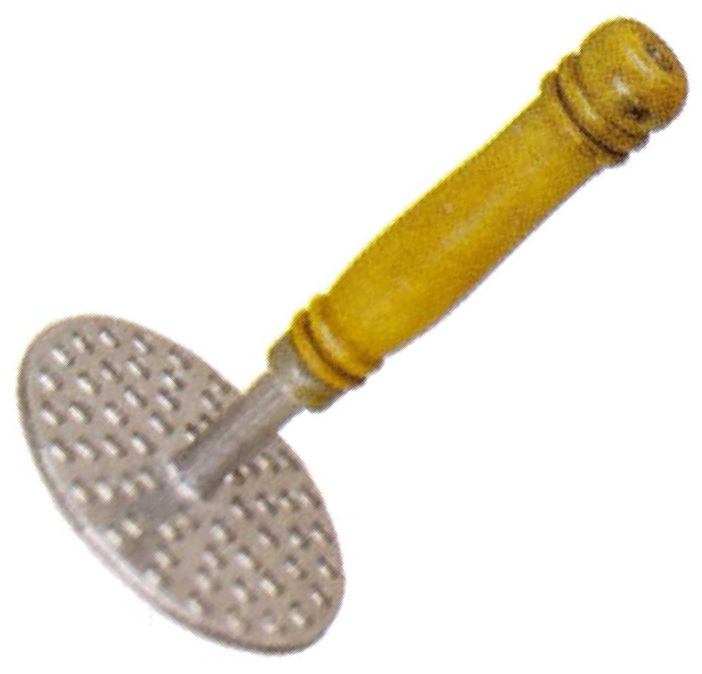
\includegraphics[scale=0.2]{pisapapas_45.png}
	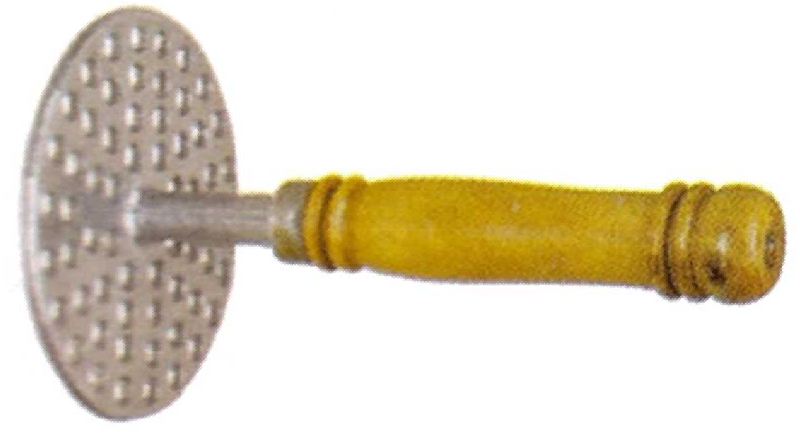
\includegraphics[scale=0.2]{pisapapas_180.png}
	
	% Fíjense que una rotación en $\R^3$ deja fija a toda una recta (el mango del pisapapas), mientras que una rotación en $\R^2$ deja fijo solo al origen. "Aumenta una dimensión" de lo que dejás quieto	
	
\end{frame}





\begin{frame}{Otro pisa papas}

	% Puede estar inclinado "en profundidad"
	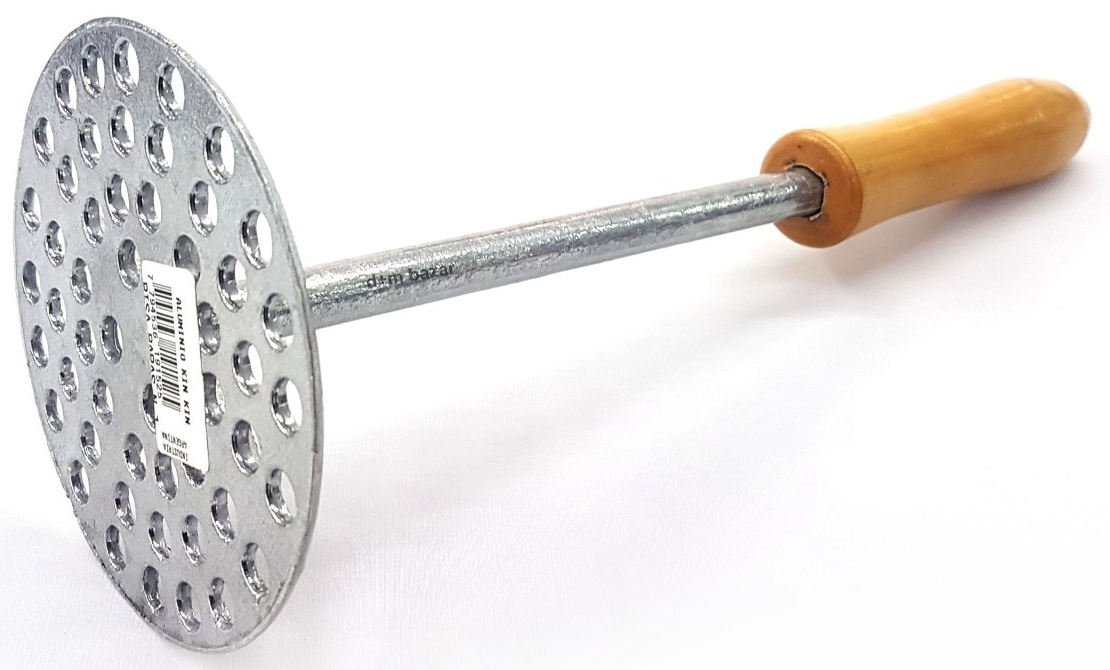
\includegraphics[scale=0.3]{pisapapas_prof.png}
	

	% Por eso son tan importantes las rotaciones en $\R^2$ para entender las que son en $\R^3$, por eso nos sirven las herramientas que aprendimos antes
	
	% Una rotación en $\R^3$ no es más que muchas rotaciones imaginarias: una por cada rejilla imaginaria - hay una por cada altura y de cada radio posible - que atraviesa de manera ortogonal al mango del pisa papas.
	
	% Entonces, ¿qué alcanza para definir una rotación en $\R^3$? En criollo pregunto.
	
	% [Pausa] ¡El mango!
\end{frame}


\begin{frame}{Por fin, cuaterniones}

	% Bueno, les presento a los cuaterniones y continuamos el jueves.
\begin{figure}  		
  	\centering
	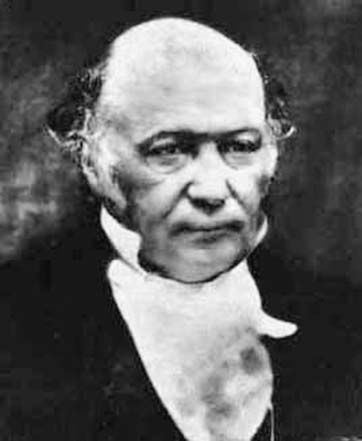
\includegraphics[scale=0.35]{images/hamilton_cara.png}
	\caption*{William Hamilton, el inventor de los horribles, \textit{horribles} cuaterniones.}
\end{figure} \pause

	% El inventor, o descubridor, si prefieren, de los cuaterniones fue un tipo que se llamaba Hamilton.
	
	% Hamilton quería generalizar el concepto de número complejo a otro objeto matemático que tuviera aplicaciones en $\R^3$
	
	% El tema es que Hamilton se imaginaba que había que agregar una sola letra imaginaria, digamos \textbf{j}. Y eso no funciona. 
Hamilton buscaba esto:
	$$a +b\cdot \textbf{i} + c \cdot \textbf{j}$$ \\
	
	($a,b,c$ son números reales) \pause
	
	...pero no funcionó.

\end{frame}

\begin{frame}

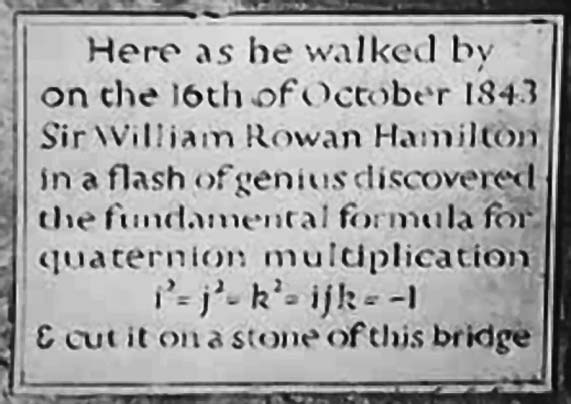
\includegraphics[scale=0.7]{images/hamilton.png}

\end{frame}

\begin{frame}{Cuaterniones}
Un cuaternión tiene esta pinta:
$$a +b\cdot \textbf{i} + c \cdot \textbf{j} + d \cdot \textbf{k}$$

	($a,b,c,d$ son números reales)  \\
	($\textbf{i},\textbf{j},\textbf{k}$ son números 'imaginarios')  \newline
	
	% Así como antes $i^2 = -1$ era la regla que usábamos para hacer cuenta, ahora estas van a ser las reglas
	

\center	Reglas:
	$$\textbf{i}^2 = \textbf{j}^2 = \textbf{k}^2 = \textbf{i}\cdot\textbf{j}\cdot\textbf{k} = -1$$ \pause 	
	% Hay algunas reglas más a tener en cuenta	
	$$\textbf{ij}=\textbf{k}\ \ \ \textbf{jk}=\textbf{i}\ \ \ \textbf{ki}=\textbf{j}$$
	$$\textbf{ji}=-\textbf{k}\ \ \ \textbf{kj}=-\textbf{i}\ \ \ \textbf{ik}=-\textbf{j}$$ \pause
	
	%O sea, i -> j -> k ->i, si multiplico dos consecutivos en orden da el otro positivo.
\end{frame}

\begin{frame}{Una representación alternativa}

Así como a un número complejo lo podíamos marcar en un plano (2 dimensiones), un cuaternión es como un vector de 4 dimensiones (no dibujable) y se puede escribir así:

$$a +b\cdot \textbf{i} + c \cdot \textbf{j} + d \cdot \textbf{k} \approx (\textbf{a},b,c,d)$$

%pero hay que tener cuidado y elegir una coordenada para que sea 'especial' ¡Fíjense que en los complejos pasaba lo mismo! La parte real era la 'especial'. Acá lo mismo.

%Se suele elegir la primera por comodidad pero tranquilamente se podría elegir otra.

\end{frame}

%TODO después de la primer charla cambiar el resumen según cómo estuvo.
\begin{frame}{Resumencito}

Los números complejos:
\begin{itemize}
	\item Se pueden marcar sumar, restar, multiplicar, dividir.
	\item Se pueden marcar en un plano.
	\item Se les puede medir la longitud y obtener el ángulo.
	\item Los de módulo $1$ representan rotaciones
	\item Para éstos, el conjugado es el inverso
	%\item Todos los complejos se pueden representar con matrices. Las matrices son el fondo funciones (transformaciones lineales)
	%\item  Algunas matrices, las que representan complejos de módulo $1$, también representan rotaciones (la función 'rotar')
\end{itemize}

\includegraphics[scale=0.4]{images/1plusi.png}

\end{frame}

\begin{frame}{Resumencito II}
\begin{itemize}
	\item Las rotaciones en $3D$ son girar alrededor de un eje por un ángulo fijo (un pisapapas).
	\item Los cuaterniones nos van a servir para representarlas.
	\item Los cuaterniones son como los complejos pero con 2 letras más y por ende más reglas que solamente $i^2=-1$.%En particular, multiplicar no siempre conmuta. Tampoco las rotaciones en $3D$.
	%\item El producto de cuaterniones es asociativo. La suma de cuaterniones es conmutativa y asociativa.
	\item Así como los complejos se pueden ver como puntos en un plano ($2D$), los cuaterniones se pueden ver como puntos de 4 dimensiones (4 números).
\end{itemize}
\end{frame}

\begin{frame}{Tarea =)}
	¿Cómo se multiplican dos cuaterniones? ¡Usar las reglas que vimos! \bigskip
	
	$$(2+3\cdot \ii + 2 \cdot \jj - 4 \cdot \kk) \cdot (1-2\cdot \ii + 1 \cdot \jj + 4 \cdot \kk) = \text{???}$$
	
	
\end{frame}

\begin{frame}{¡Fin!}
\Huge ¿Preguntas?
\end{frame}



\iffalse

\begin{frame}{¡Cuidado!}
Ojo: El producto de cuaterniones en general no es conmutativo.

	% Fíjense que el producto NO es conmutativo en este caso.
	% Déjenme justificarles por qué el producto no es conmutativo de una manera intuitiva

	% Si los cuaterniones están relacionados con las rotaciones en $\R^3$ (lo vamos a ver la próxima clase) tiene sentido que si las rotaciones no son conmutativas entonces el producto de cuaterniones tampoco.
	
	% Las rotaciones en $\R^3$, ¿son conmutativas?
	
	% No. Y lo podemos ver con un cubo de rubik. Las rotaciones en $\R^3$ no son lo mismo que las de un cubo de rubik, pero sirven para generar intuición.
	
	% Si rotamos para abajo y para la izquierda no queda igual que primero para la izquierda y después para abajo.
	
	% Esto ya nos da una primer diferencia con $\R^2$
\end{frame}

\fi

\end{document}
